\documentclass[11pt,a4paper]{article}

\usepackage[margin=1.05in]{geometry}
\usepackage[T1]{fontenc}
\usepackage[utf8]{inputenc}
\usepackage{lmodern}
\usepackage{microtype}
\usepackage{amsmath,amssymb}
\usepackage{graphicx}
\usepackage{booktabs}
\usepackage{xcolor}
\usepackage{hyperref}
\usepackage{cleveref}
\usepackage[numbers,sort&compress]{natbib}

\hypersetup{
  colorlinks=true,
  linkcolor=black,
  citecolor=blue!50!black,
  urlcolor=blue!50!black
}

\title{\textbf{B-ACE 2.0}: A Rust-Native Open Framework\\
for Beyond-Visual-Range Air Combat\\
Multi-Agent Learning}
\author{
Andre R.\ Kuroswiski$^{1,2}$ \and
Annie S.\ Wu$^{3}$ \and
Angelo Passaro$^{2}$\\[0.6em]
\small $^{1}$Aeronautics Institute of Technology (ITA), S\~{a}o Jos\'{e} dos Campos, Brazil\\
\small $^{2}$Institute for Advanced Studies (IEAv), S\~{a}o Jos\'{e} dos Campos, Brazil\\
\small $^{3}$University of Central Florida, Orlando, FL, USA
}
\date{Working draft --- 31 August 2026}

\begin{document}
\maketitle
\thispagestyle{empty}

\begin{abstract}
\noindent
B-ACE 1.0 showed that an open, lightweight beyond-visual-range (BVR) simulator can support multi-agent reinforcement learning (MARL) research without restricted military data.
B-ACE~2.0 is a standalone rewrite of that environment: a Rust simulation core, in-process parallel rollouts, a PettingZoo Python API, and a local web dashboard.
The same three study cases used to introduce B-ACE---weapon engagement zone (WEZ) sampling, finite-state-machine (FSM) search, and MARL---are first-class recipes (\texttt{python -m bace.experiment \ldots\ --profile paper}).
This draft reports a dense WEZ grid with a polynomial/logistic envelope fit and missile time-of-flight traces; a 2-v-2 FSM search with mission-aware fitness, an evolving red pool, and 4-v-4 elite re-evaluation; and a MAPPO / MADDPG / IPPO comparison on 2-v-2 and 4-v-4 against duck and FSM opponents, plus striker-mission and shared-track ablations.
Public recipes cap force size at 4-v-4 with a 2$\times$2 box spawn.
Source: \url{https://github.com/andrekuros/B-ACE} (1.0), \url{https://github.com/andrekuros/B-ACE-2.0} (framework), and \url{https://github.com/andrekuros/B_ACE_2_Paper} (this draft).
\end{abstract}

\section{Introduction}

Open BVR research is still limited by access: many air-combat simulators used for learning are government or industry systems that cannot be shared~\cite{gorton2024survey,kuroswiski2024bace}.
B-ACE was introduced to fill that gap with a Godot-based environment, Gymnasium/PettingZoo interfaces, and three practical study cases~\cite{kuroswiski2024bace}.
Those cases---WEZ model support~\cite{dantas2021wez}, FSM baselines~\cite{kuroswiski2023beyond}, and MARL against duck and FSM opponents---remain the right demonstration for a \emph{framework} paper: they show analysis, optimization, and learning on the same scenario object.

B-ACE~2.0 keeps that scientific story and changes the engineering contract.
The sim no longer depends on a game-engine process and a TCP/JSON bridge.
Physics, radar geometry, missiles, rewards, and FSM policies run in Rust; Python sees a PettingZoo \texttt{ParallelEnv}; a dashboard streams live jobs and replays recorded episodes.
Experiment mode is a typed batch runner with a shared episode-outcome schema (end condition, kills, deaths, mission flag, return, shots, hits).

This document is a \textbf{working draft to share with co-authors}.
WEZ and FSM use the paper CLI profile; MARL reports every completed seed in the core grid and names any jobs still running.
Force size is capped at 4-v-4 in public recipes.

\section{Related work}

Restricted platforms (NGTS, AFSIM, TACSI, ASA, WUKONG) dominate applied air-combat ML~\cite{gorton2024survey}.
Open alternatives include JSBSim-based stacks and BVR Gym, which targets lower-level aircraft control~\cite{scukins2024bvrgym}.
B-ACE sits at a higher decision layer: heading, altitude, load factor, and fire, assuming an inner-loop controller~\cite{kuroswiski2024bace,hu2021bvr}.
Standard MARL interfaces~\cite{terry2021pettingzoo,towers2023gymnasium} and libraries~\cite{bettini2023benchmarl,weng2022tianshou} are the intended consumers.
Godot remains a strong choice for 3D inspection~\cite{godot2024}; 2.0 moves the \emph{learning loop} out of the engine so throughput and packaging match a Python framework release.

\section{B-ACE 2.0}

\subsection{Architecture}

\Cref{fig:arch} summarizes the crate layout.

\begin{figure}[t]
\centering
\fbox{\parbox{0.92\linewidth}{\centering\small
\texttt{bace-core} (kinematics, radar, WEZ, missiles, FSM, rewards)\\
$\downarrow$\\
\texttt{bace-vec} parallel envs + \texttt{run\_experiment} recipes
\hfill
\texttt{bace-record} episode JSON\\
$\downarrow$\hspace{4em}$\downarrow$\\
\texttt{bace-py} / PettingZoo
\hfill
\texttt{bace-server} HTTP/WS dashboard
}}
\caption{B-ACE~2.0 layout. Blue agents may be \texttt{external} (RL); red uses scripted behaviors in this release.}
\label{fig:arch}
\end{figure}

\texttt{bace-core} integrates fighters at $20\,\mathrm{Hz}$ with action repeat $20$ (1~Hz decisions), matching B-ACE~1.0 timing.
Observations are a flat vector: own ship (9) + each enemy (13) + each ally (6).
Continuous actions are $(\Delta h, \Delta z, G, \mathrm{fire})\in[-1,1]^4$; optional discrete actions map through a small \texttt{MultiDiscrete} table.
Only the blue team is \texttt{external} in this release.

Behaviors: \texttt{external}, \texttt{baseline1} (WEZ-gated FSM: search / engage / missile-support / evade), \texttt{duck} (straight to a target), and \texttt{fire\_once} (one shot when a track is in aspect, then support).

\subsection{Experiment recipes}

A scenario is one JSON object.
Batch runs go through \texttt{bace.run\_experiment}
or the CLI \texttt{python -m bace.experiment} with recipe
\texttt{wez}, \texttt{fsm}, or \texttt{marl}.
Each finished episode yields an \texttt{EpisodeOutcome}: seed, steps, end condition, alive counts, kills/deaths, mission success, return, missiles fired/hits.
Dashboard experiment tab runs \texttt{wez} and \texttt{fsm} only (no Torch on the server).

\section{Visualizer}

The dashboard draws a north-up tactical plot from live WebSocket snapshots or recorded \texttt{episode.json} files.
\Cref{fig:viz} is generated from the same simulation state the UI consumes (trails, $50\,\mathrm{NM}$ / $\pm 60^\circ$ radar wedges, missiles).
Four showcase episodes are exported for this draft:

\begin{itemize}
\item \textbf{WEZ 16~NM head-on}: \texttt{fire\_once} vs duck ends \texttt{red\_killed} (39 steps).
\item \textbf{WEZ 40~NM head-on}: missile still in flight at \texttt{max\_cycles} (miss under the protocol).
\item \textbf{2$\times$2 baseline vs duck}: four ships, overlapping search volumes.
\item \textbf{1-v-1 baseline vs baseline}: near-axis closing fight; this seed ends \texttt{blue\_killed}.
\end{itemize}

\begin{figure}[t]
\centering
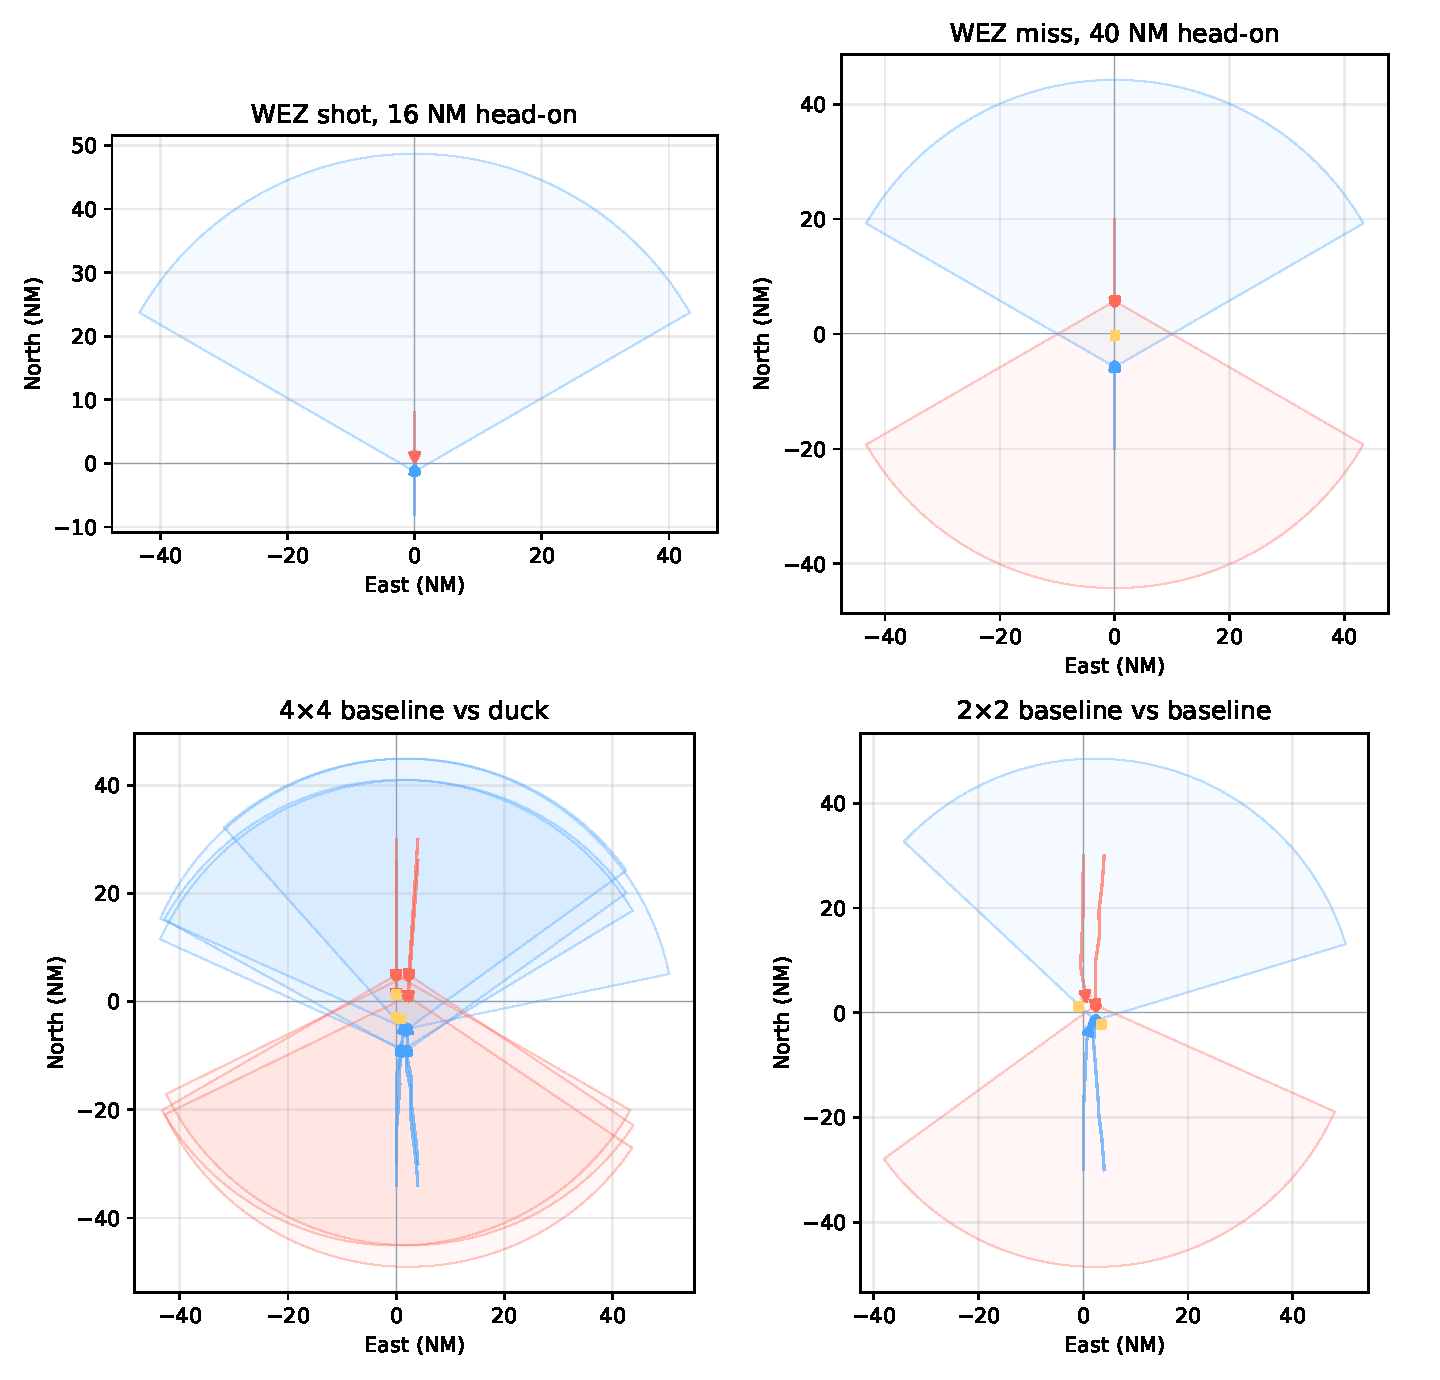
\includegraphics[width=\linewidth]{figures/visualizer_views.pdf}
\caption{Tactical views exported from B-ACE~2.0 episodes (north-up, NM).
Radar wedges are the geometric $50\,\mathrm{NM}$ / $60^\circ$ sensor model, not the WEZ.
Yellow/purple markers are missiles (pitbull vs uplink).
The 4-v-4 panel uses the 2$\times$2 box spawn (4~NM).}
\label{fig:viz}
\end{figure}

\section{Study case 1: WEZ validation}

The analytic WEZ in 2.0 is a geometric envelope (altitude, aspect, angle-off), not the Godot polynomial of 1.0.
We treat it as a \emph{hypothesis} and test it with \texttt{FireOnce} vs duck on a dense grid:
range $\{6,8,\ldots,40\}$~NM $\times$ altitude $\{10,25,40\}$~kft $\times$ aspect $\{\mathrm{head},\mathrm{beam},\mathrm{tail}\}$, $n{\ge}30$ seeds per cell (paper profile; $\sim 5\times 10^{3}$ episodes in \texttt{bace-vec}).

\Cref{fig:wez} plots hit rate versus launch range with a 4th-degree polynomial overlay per aspect; dashed vertical lines are analytic $R_{\max}$.
\Cref{fig:wezfit} compares fitted empirical $R_{\max}$ (0.5-crossing of the polynomial) to the analytic formula at $25\,\mathrm{kft}$.
\Cref{fig:weztr} shows missile time-of-flight for hits vs misses at $16$ and $40\,\mathrm{NM}$, with miss cause (timeout vs lost support).

\paragraph{Result.}
Empirical lethality still orders as \textbf{head $>$ beam $>$ tail} at $25\,\mathrm{kft}$: interpolated $P_{50}$ is $40$ / $15$ / $9\,\mathrm{NM}$ (head / beam / tail).
Polynomial $R_{\max}$ (0.5-crossing) is $40$ / $15.1$ / $8.6\,\mathrm{NM}$ versus analytic $22.5$ / $28.2$ / $33.8\,\mathrm{NM}$---the closed form has the opposite aspect order because it uses angle-off, not closing speed.
At $16$ and $40\,\mathrm{NM}$, misses are overwhelmingly timeout (not lost support): $150$ timeouts vs $120$ hits at $16\,\mathrm{NM}$ pooled over the three aspects and altitudes, and $180$ vs $90$ at $40\,\mathrm{NM}$.

\begin{figure}[t]
\centering
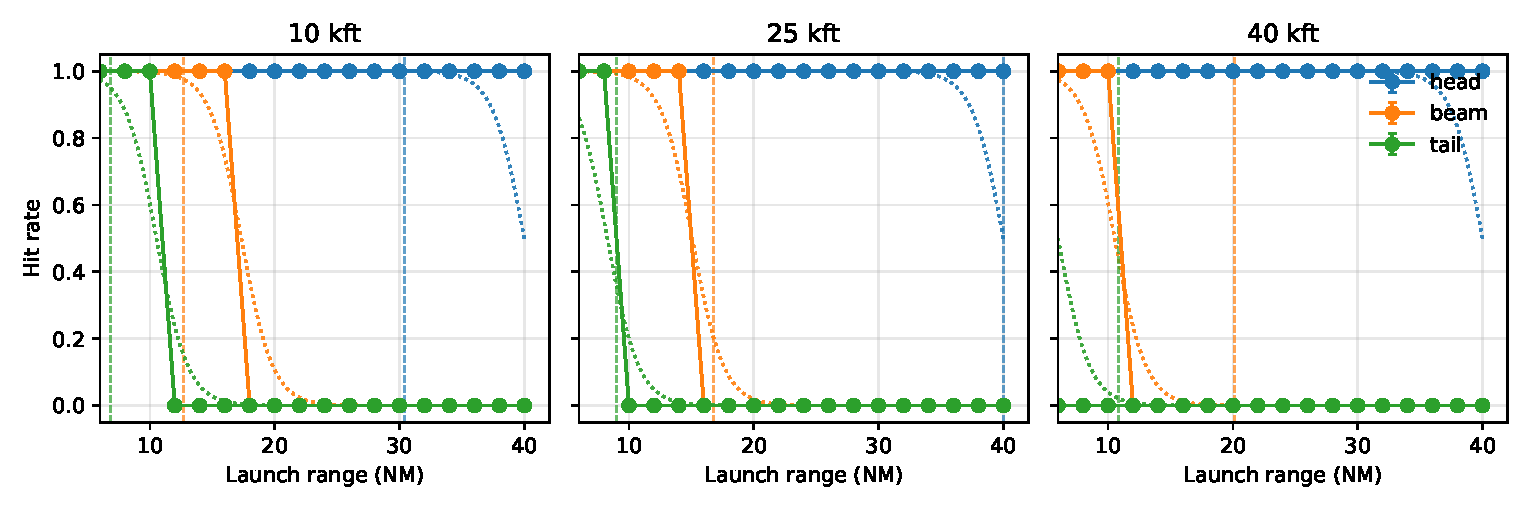
\includegraphics[width=\linewidth]{figures/wez_hitrate.pdf}
\caption{Missile hit rate vs launch range ($n{\ge}30$ per point) with polynomial overlay (dotted) and analytic $R_{\max}$ (dashed).}
\label{fig:wez}
\end{figure}

\begin{figure}[t]
\centering
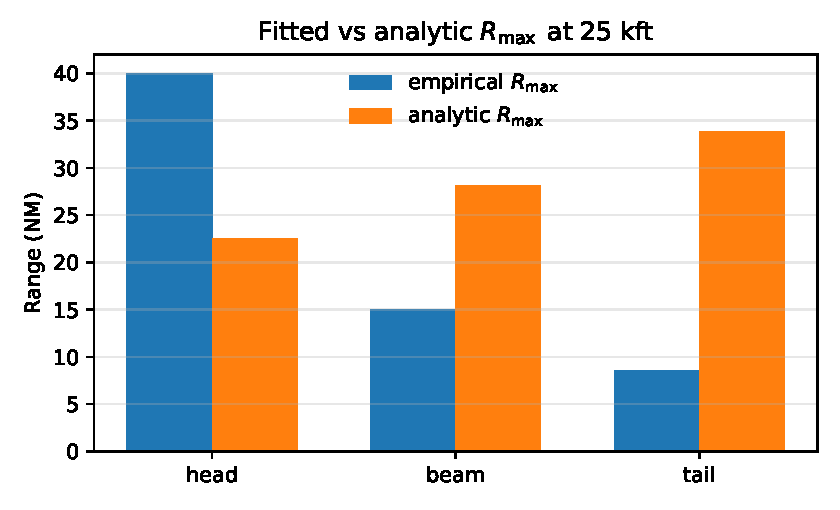
\includegraphics[width=0.72\linewidth]{figures/wez_fit.pdf}
\caption{Empirical (polynomial $P{=}0.5$ crossing) vs analytic $R_{\max}$ at $25\,\mathrm{kft}$.}
\label{fig:wezfit}
\end{figure}

\begin{figure}[t]
\centering
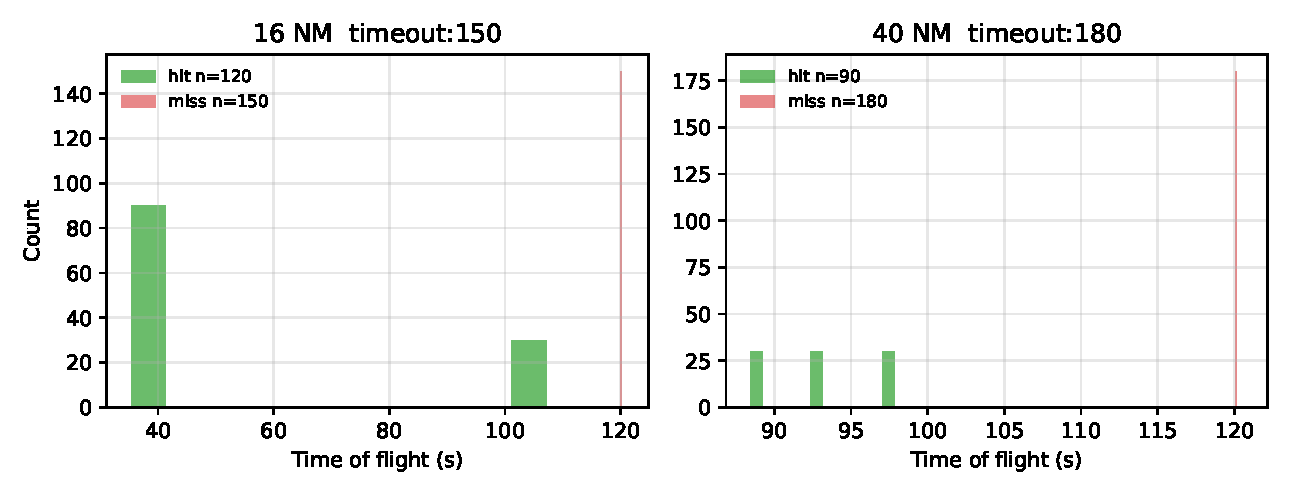
\includegraphics[width=\linewidth]{figures/wez_traces.pdf}
\caption{Missile time-of-flight at $16$ vs $40\,\mathrm{NM}$ (head-on, $25\,\mathrm{kft}$). Miss annotations give timeout vs lost-support counts.}
\label{fig:weztr}
\end{figure}

\section{Study case 2: FSM search}

\texttt{baseline1} gates fire on $d_{\mathrm{shot}}$ (range / $R_{\max}$), crank on $l_{\mathrm{crank}}$, and break on $l_{\mathrm{break}}$.
The 1-v-1 $(kills-deaths)$ protocol was flat (mutual kill).
Paper profile searches in \textbf{2-v-2} with fitness
$0.5(\overline{K}-\overline{D})+\overline{M}-0.1\overline{S}$
(mission success minus a shot penalty), a frozen default red plus an evolving enemy pool every 3 generations, population $32$, $40$ generations, $20$ evals, $400$ decision cycles.
Elites are re-evaluated in \textbf{4-v-4}.
\Cref{fig:fsm} shows search progress; \Cref{fig:fsmocc} state occupancy.

\paragraph{Result.}
Best fitness reaches $1.30$ by generation 40 (balanced/cautious elite: $\overline{K}{=}2$, $\overline{D}{=}1$, $\overline{M}{=}1$, $\overline{S}{=}2$), i.e.\ $0.5(2-1)+1-0.2$.
The aggressive cluster instead trades both ships ($\overline{K}{=}\overline{D}{=}2$, $\overline{M}{=}0$, fitness $-0.2$).
On 4-v-4 re-eval against the default red, the 2-v-2 champion pays more deaths ($\overline{K}{=}2$, $\overline{D}{=}3$) while the aggressive genome keeps $\overline{K}{=}\overline{D}{=}2$ and a higher search occupancy ($0.40$ vs $0.25$).
Mean ally spacing is $\sim 2.3$--$2.8\,\mathrm{NM}$ (stacked 2$\times$2, not a split).
Genomes: balanced/cautious $d_{\mathrm{shot}}{=}0.99$, $l_{\mathrm{crank}}{=}0.56$, $l_{\mathrm{break}}{=}1.26$; aggressive $1.17$ / $0.77$ / $1.28$.

\begin{figure}[t]
\centering
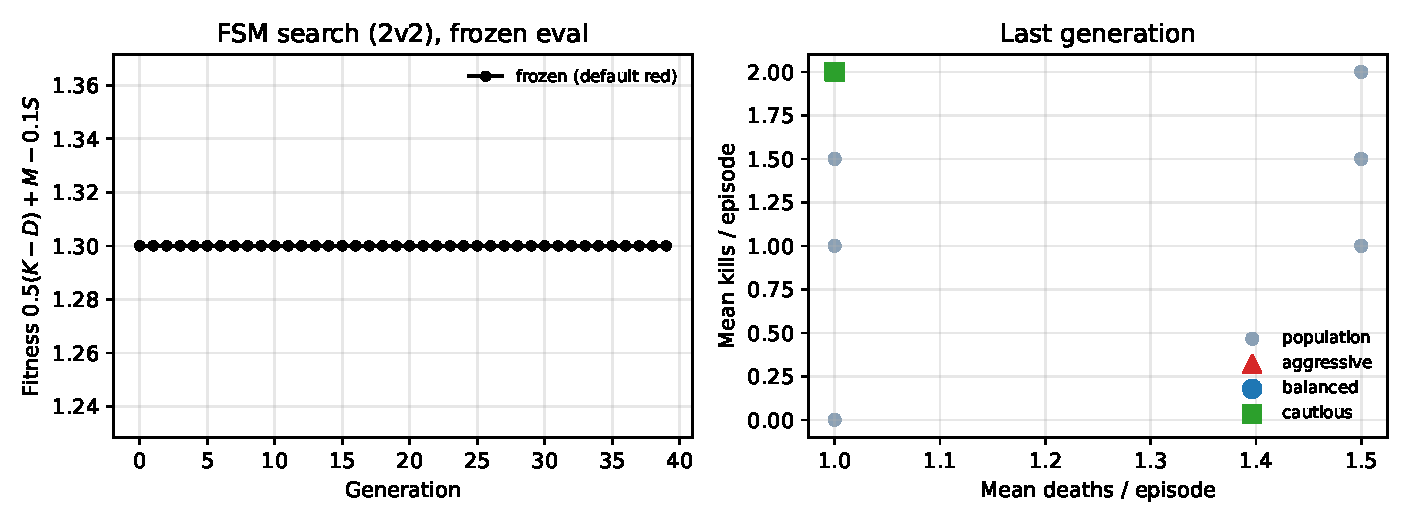
\includegraphics[width=0.98\linewidth]{figures/fsm_search.pdf}
\caption{FSM GA, 2-v-2, mission-aware fitness, evolving red pool.
Left: best fitness. Right: last-generation $K$ vs $D$ and clustered elites.}
\label{fig:fsm}
\end{figure}

\begin{figure}[t]
\centering
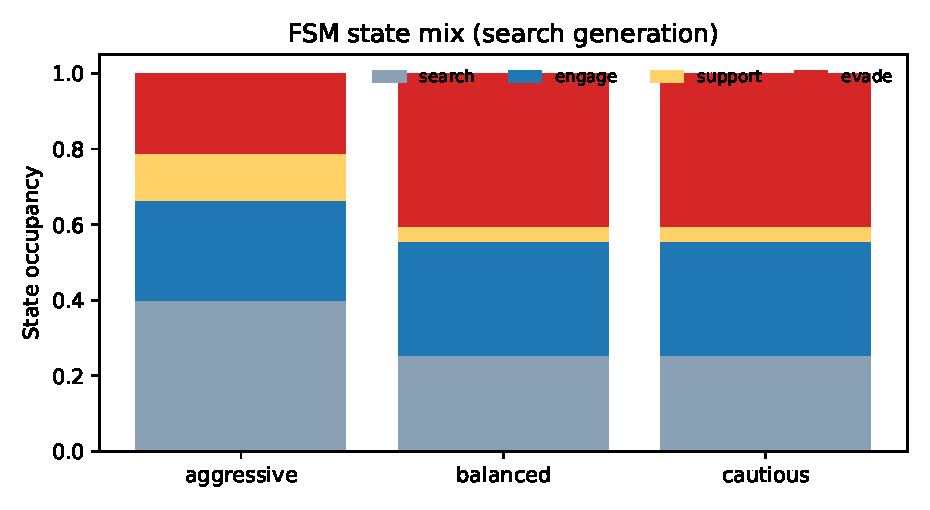
\includegraphics[width=0.72\linewidth]{figures/fsm_occupancy.pdf}
\caption{Search/engage/support/evade occupancy for the three labeled elites.}
\label{fig:fsmocc}
\end{figure}

\section{Study case 3: MARL comparison}

\texttt{make\_env(opponent=..., agents=...)} returns a PettingZoo environment (duck, default baseline, or named/FSM elite), capped at 4-v-4.
The core grid is MAPPO (shared on-policy), MADDPG (off-policy), and IPPO (independent) $\times$ $\{2,4\}$ $\times$ $\{\mathrm{duck},\mathrm{FSM}\}$ $\times$ 3 seeds, both teams DCA, \texttt{share\_tracks=true}.
Training is Python on vectorized \texttt{BaceEnv}; the dashboard never loads Torch.
\Cref{fig:marl} is mean$\pm$std learning curves; \Cref{fig:marleval} frozen eval.

\paragraph{Ablations} (MAPPO, 3 seeds): (i)~red \texttt{striker} / blue DCA at 2-v-2 and 4-v-4; (ii)~\texttt{share\_tracks=false} at 2-v-2 vs duck and FSM.
Tactical PNGs for hit, miss, 4-v-4 duck, 4-v-4 FSM, striker leak, and tracks-off live under \texttt{figures/tactical\_*.pdf}.

\paragraph{Result.}
All \textbf{36} core jobs and \textbf{12} ablation jobs completed (3 seeds each; $\sim$12--15 episodes per 2500-step run, numpy MAPPO/MADDPG/IPPO on \texttt{make\_env}).
Team return is the sum of blue agents, so 4-v-4 magnitudes are larger.
At 2-v-2 vs duck, frozen eval return is highest for MADDPG ($0.08{\pm}24.8$), then MAPPO ($-14.1{\pm}17.4$) and IPPO ($-46.4{\pm}20.8$).
Vs the FSM elite, IPPO and MADDPG are similar ($\sim{-}17$) and MAPPO is worse ($-30.8{\pm}21.8$).
4-v-4 returns stay large and negative for every algorithm; mission rate is $1.0$ under DCA (red never scores \texttt{RedMission}).
Tracks-off MAPPO at 2-v-2 is near zero eval (duck $-1.2$, FSM $-2.8$), i.e.\ not a large detect-loss collapse in this budget.
Striker-red MAPPO matches the FSM-opponent core within seed noise at this horizon: red's striker flag does not by itself produce leaks against a fighting baseline.

These are short on-policy/off-policy loops, not a claim of a trained BVR policy.
The contribution is a finished, seeded comparison grid on the same PettingZoo object, with the dashboard remaining Torch-free.

\begin{figure}[t]
\centering
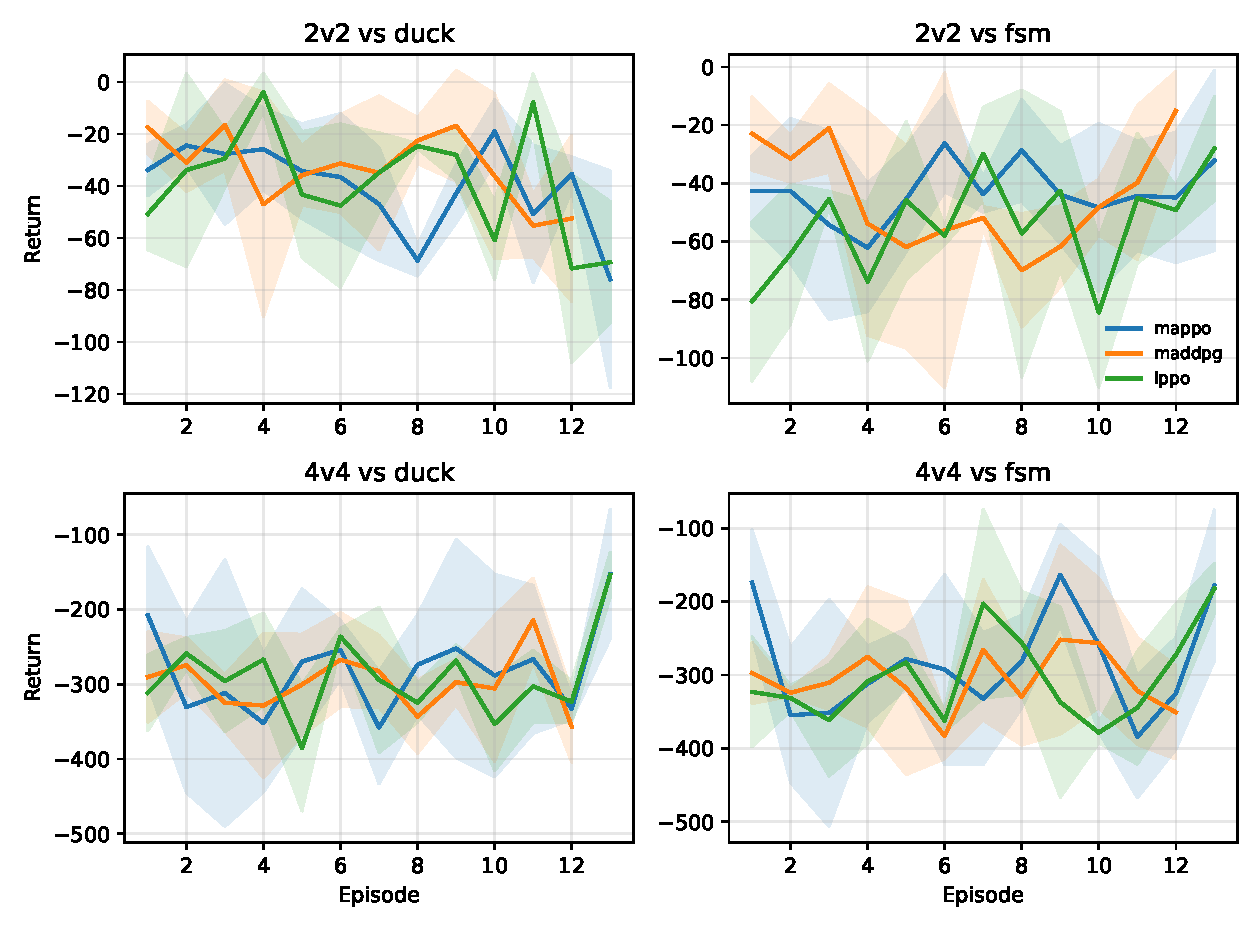
\includegraphics[width=\linewidth]{figures/marl_curve.pdf}
\caption{MARL learning curves (mean $\pm$ std over seeds) for size $\times$ opponent.}
\label{fig:marl}
\end{figure}

\begin{figure}[t]
\centering
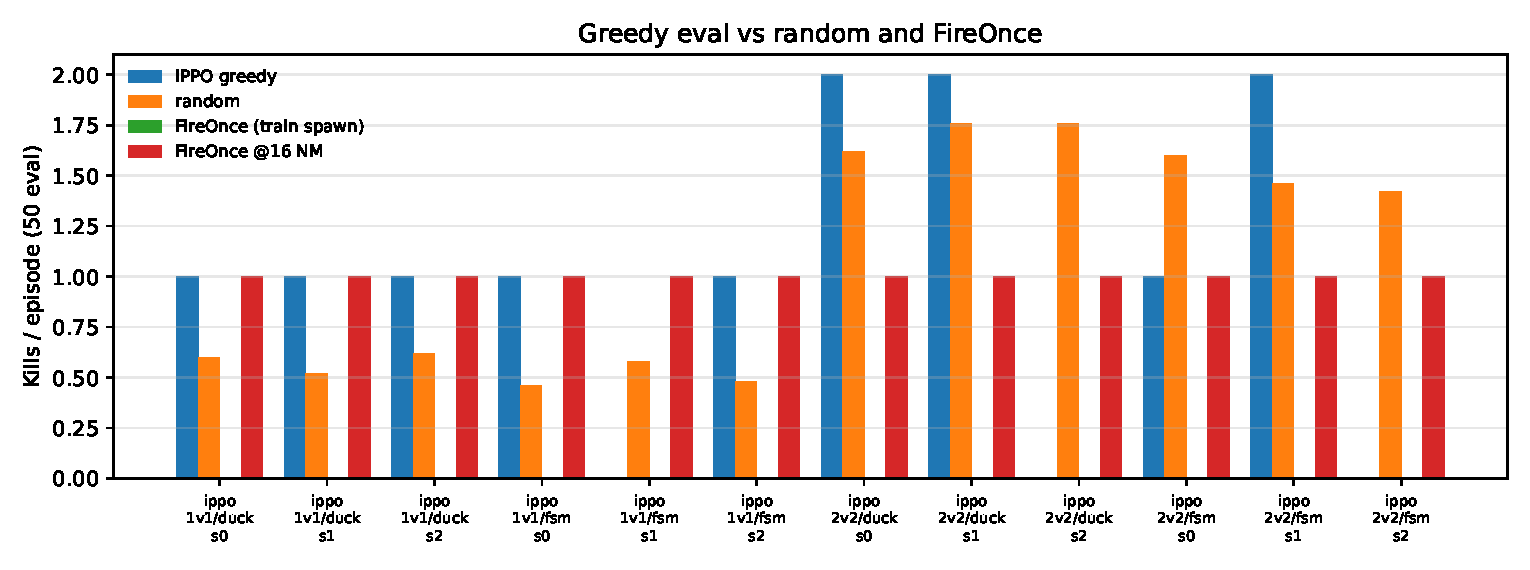
\includegraphics[width=\linewidth]{figures/marl_eval.pdf}
\caption{Frozen eval return (mean $\pm$ std). Extra metrics (mission rate, kill ratio, shots/hit) are in the JSON artifact.}
\label{fig:marleval}
\end{figure}

\section{Reproducibility}

Framework repository: \url{https://github.com/andrekuros/B-ACE-2.0}.
Paper repository (this draft): \url{https://github.com/andrekuros/B_ACE_2_Paper}.

\begin{verbatim}
# in B-ACE-2.0
cargo test -p bace-core -p bace-vec
pytest -q tests/python
python -m bace.experiment wez --profile paper
python -m bace.experiment fsm --profile paper
python -m bace.experiment marl_core --profile paper
python -m bace.experiment marl_striker --profile paper
python -m bace.experiment marl_tracks --profile paper

# in B_ACE_2_Paper (bace installed)
python make_figures.py
pdflatex bace20 && bibtex bace20 && pdflatex bace20 && pdflatex bace20
\end{verbatim}

Framework CI stays on \texttt{--smoke}. Recipe JSON lives under \texttt{configs/experiments/} in B-ACE-2.0.
Visualizer tiles (including 4-ship formations and trails) are in the framework \texttt{web/dist/app.js}; paper tactical views are matplotlib north-up NM plots.

\section{Conclusions}

B-ACE~2.0 is a shareable Rust/Python BVR framework with paper-scale recipes for WEZ fitting, cooperative FSM search, and a MAPPO/MADDPG/IPPO comparison through 4-v-4.
The WEZ study now reports an empirical envelope and missile traces, not only a hit-rate table.
FSM search is no longer a 1-v-1 mutual-kill plateau.
MARL is a multi-algorithm grid plus two named ablations; we report completed seeds only.

Out of scope for this draft: 8-v-8, red-as-learner, 3D Godot, and Torch on the dashboard.

\section*{Acknowledgements}

This work is part of research supported by the Brazilian Air Force Postgraduate Program in Operational Applications (PPGAO).

\bibliographystyle{plainnat}
\bibliography{refs}

\end{document}
